\documentclass[conference]{IEEEtran}
\usepackage{fontspec}
\setmainfont{texgyretermes-regular.otf}[BoldFont=texgyretermes-bold.otf,ItalicFont=texgyretermes-italic.otf,BoldItalicFont=texgyretermes-bolditalic.otf]
\usepackage{cite}
\usepackage{balance}
\usepackage{amsmath}
\usepackage{graphicx}
\usepackage{booktabs}
\usepackage{array}
\usepackage{url}
\renewcommand{\abstractname}{Tóm tắt}
\renewcommand{\IEEEkeywordsname}{Từ khóa}
\renewcommand{\figurename}{Hình}
\renewcommand{\tablename}{Bảng}
\renewcommand{\appendixname}{Phụ lục}
\renewcommand{\refname}{Tài liệu tham khảo}
\newcommand{\rqRuns}{3}
\newcommand{\rqFullAcc}{97,894 $\pm$ 0,004}
\newcommand{\rqFullPrec}{91,93 $\pm$ 0,80}
\newcommand{\rqFullRec}{84,43 $\pm$ 0,55}
\newcommand{\rqFullFone}{86,42 $\pm$ 0,45}
\newcommand{\rqFullFpr}{0,245 $\pm$ 0,006}
\newcommand{\rqFullFnr}{5,787 $\pm$ 0,018}
\newcommand{\rqDedupAcc}{98,189 $\pm$ 0,011}
\newcommand{\rqDedupPrec}{83,15 $\pm$ 1,59}
\newcommand{\rqDedupRec}{76,78 $\pm$ 0,64}
\newcommand{\rqDedupFone}{78,78 $\pm$ 0,92}
\newcommand{\rqDedupFpr}{0,279 $\pm$ 0,004}
\newcommand{\rqDedupFnr}{6,908 $\pm$ 0,024}
\newcommand{\rqDupShare}{27,8}


\begin{document}

\title{Dùng lời giải thích để chẩn đoán lối tắt của bộ dữ liệu trong hệ thống phát hiện xâm nhập mạng trực tuyến}

\author{\IEEEauthorblockN{Nguyễn Thanh Sơn, Nguyễn Tùng Dương, Tăng Khánh Nhi và Võ Ngọc Bảo Vy}
\IEEEauthorblockA{Trường Đại học FPT, Việt Nam}}

\maketitle

\begin{abstract}
Hệ thống phát hiện xâm nhập dùng học máy thường được đánh giá bằng độ chính xác trên một bộ dữ liệu công khai. Chúng tôi báo cáo một trường hợp trong đó điểm số cao che giấu một lối tắt. Bộ phân loại XGBoost huấn luyện trên CSE-CIC-IDS2018, gọi là M0, đạt độ chính xác 97,9\% trên tập kiểm thử của nó, nhưng báo tấn công trên 149 trong 784 flow (19,0\%, khoảng tin cậy 95\% từ 16,4 đến 21,9) mà chúng tôi thu trên một máy tính Windows và xác nhận là bình thường. Giá trị SHAP, vết đường đi quyết định trong cây và các phép thử đổi từng đặc trưng một cùng chỉ về cờ FIN của TCP. Một vùng trong không gian đặc trưng xác định bằng ba điều kiện, gọi là vùng FIN, chứa 148 trong 149 cảnh báo trên các flow thực và 99,97\% cảnh báo sai trên một tập kiểm thử lớn gồm flow bình thường có nhãn. Trong dữ liệu huấn luyện gốc, vùng này chỉ chứa flow DoS-Hulk. Hiện tượng phù hợp với một bộ trích xuất flow cắt flow tại gói FIN đầu tiên, như các nghiên cứu trước báo cáo cho những bộ dữ liệu liên quan, nhưng chúng tôi không kiểm tra được điều này trên gói tin thô. Bộ phân loại thứ hai, M1, huấn luyện theo cùng cách trên dữ liệu dựng lại với nhãn đã sửa, không đưa ra cảnh báo nào trên 784 flow, với cận trên 95\% là 0,47\%. Bộ dữ liệu đã sửa chứa các flow gần trùng nhau, nên độ chính xác 99,99\% của nó không dự báo hiệu năng ngoài thực tế. Trong cấu hình đã thử, LIME không cho độ khớp cục bộ hợp lệ trên flow thật, còn TreeSHAP đạt kiểm tra cộng dồn trên mọi flow. Bài mô tả hệ thống trực tuyến cung cấp lời giải thích và báo cáo độ trễ của hệ thống.
\end{abstract}

\begin{IEEEkeywords}
phát hiện xâm nhập, trí tuệ nhân tạo có thể giải thích, SHAP, LIME, XGBoost, chất lượng bộ dữ liệu, học lối tắt
\end{IEEEkeywords}

\section{Giới thiệu}
Một hệ thống phát hiện xâm nhập dùng học máy thường được huấn luyện và kiểm thử trên cùng một bộ dữ liệu công khai, và độ chính xác trên tập kiểm thử được coi là thước đo chất lượng. CSE-CIC-IDS2018 \cite{sharafaldin2018} là một trong những bộ dữ liệu được dùng theo cách này. Liu và cộng sự mô tả nó là một bộ chuẩn chính cho phát hiện xâm nhập mạng \cite{liu2022}. Chính nhóm tác giả này, và trước đó là Engelen và cộng sự, đã tìm thấy lỗi trong cách các bộ dữ liệu này được xây dựng \cite{engelen2021,liu2022}. Người huấn luyện trên dữ liệu như vậy không thể biết từ điểm kiểm thử liệu một lỗi đã đi vào mô hình hay chưa.

Chúng tôi gặp vấn đề này khi xây dựng một bộ phát hiện trực tuyến. Công việc đi theo bốn câu hỏi nghiên cứu, và mỗi câu hỏi dựa vào câu trả lời của câu trước.
\begin{itemize}
\item \textbf{RQ1.} Bộ phân loại XGBoost \cite{chen2016} phát hiện tấn công tốt đến đâu trên CSE-CIC-IDS2018? Mô hình thu được gọi là M0.
\item \textbf{RQ2.} Phương pháp giải thích nào, SHAP \cite{lundberg2017,lundberg2020} hay LIME \cite{ribeiro2016}, phù hợp với bộ phát hiện này?
\item \textbf{RQ3.} Bộ phát hiện và lời giải thích có chạy được trong một hệ thống trực tuyến không, và bộ phát hiện hành xử ra sao trên lưu lượng thật?
\item \textbf{RQ4.} Lời giải thích có truy được một lỗi thấy ở RQ3 về một lối tắt trong dữ liệu huấn luyện không, và huấn luyện lại trên dữ liệu đã sửa có loại bỏ lỗi đó không? Mô hình huấn luyện lại gọi là M1.
\end{itemize}

Các câu trả lời tạo thành một câu chuyện, trong đó mỗi kết quả dẫn đến câu hỏi kế tiếp. Ở RQ1, M0 đạt độ chính xác 97,9\%, nên chúng tôi giữ nó. Chỉ có nhãn thì người phân tích không biết vì sao một flow bị báo, nên RQ2 so sánh các cách giải thích và SHAP tốt hơn. Ở RQ3, chúng tôi triển khai M0 cùng SHAP, và M0 báo tấn công trên lưu lượng bình thường từ chính máy tính của chúng tôi, điều mà điểm chuẩn không dự báo. RQ4 hỏi vì sao. SHAP và vết đường đi quyết định đã xác định một lối tắt dữ liệu có khả năng là nguyên nhân, và huấn luyện lại trên dữ liệu đã sửa đã loại bỏ mẫu cảnh báo sai quan sát được. Hình~\ref{fig:chain} cho thấy chuỗi bằng chứng.

M0 là bộ phát hiện đã thất bại. Nó được huấn luyện trên dữ liệu gốc. M1 dùng cùng thuật toán, cùng thiết lập và cùng cách lấy mẫu, và được huấn luyện trên một phiên bản đã sửa của cùng bộ dữ liệu \cite{liu2022}. Chúng tôi huấn luyện M1 vì một lý do, đó là kiểm tra lời giải thích. Nếu lối tắt đến từ dữ liệu huấn luyện, mô hình huấn luyện trên dữ liệu đã sửa sẽ không còn nó. Nếu M1 vẫn báo tấn công trên cùng lưu lượng, nguyên nhân nằm ở nơi khác, chẳng hạn ở các đặc trưng hoặc ở chính lưu lượng. Giữa M0 và M1, thuật toán và thiết lập giữ nguyên, còn dữ liệu huấn luyện thay đổi ở bộ trích xuất, nhãn và tập lớp.

Bài báo có ba đóng góp.
\begin{itemize}
\item Bài ghi lại một trường hợp trong đó lối tắt của một bộ dữ liệu xâm nhập công khai gây ra tỷ lệ cảnh báo 19\% trên lưu lượng đã xác nhận là bình thường, trong khi độ chính xác trên bộ chuẩn là 97,9\%.
\item Bài đưa ra một quy trình chẩn đoán ngắn gồm giá trị SHAP, vết đường đi quyết định, kiểm tra vùng trên dữ liệu thu sau, các phép thử độ nhạy khi can thiệp một đặc trưng và kiểm tra dữ liệu huấn luyện.
\item Bài kiểm tra cách sửa và nêu giới hạn của nó. Mô hình huấn luyện lại không báo cảnh báo nào trên các flow đã xác nhận bình thường, nhưng bộ chuẩn của nó dễ, LIME không cho độ khớp hợp lệ trên flow thật trong thiết lập của chúng tôi, và hệ thống làm việc ở mức flow đã hoàn tất.
\end{itemize}

\begin{figure*}[t]
\centering
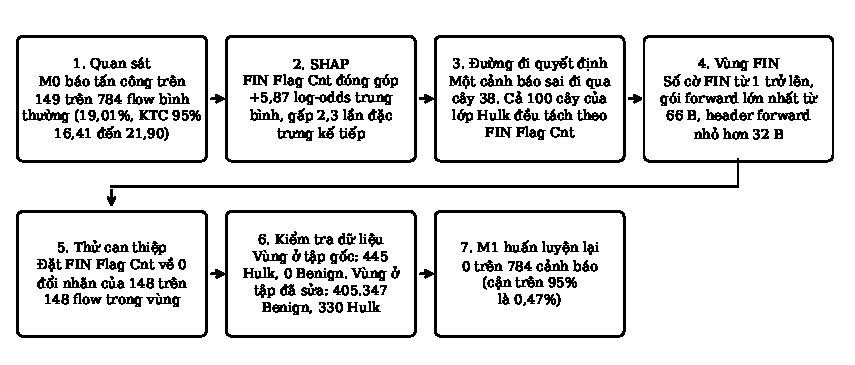
\includegraphics[width=0.92\textwidth]{figures_vi/fig1_chain.pdf}
\caption{Chuỗi bằng chứng của bài. Các bước 1 đến 3 và bước 5 dùng 784 flow thực hoặc 148 flow trong vùng FIN thuộc tập đó. Bước 4 được kiểm chứng trên dữ liệu thu sau, và bước 6 dùng các tập huấn luyện. Bước 7 dùng lại 784 flow thực với M1.}
\label{fig:chain}
\end{figure*}

\section{Các nghiên cứu liên quan}
\subsection{Chất lượng của các bộ dữ liệu CIC}
CSE-CIC-IDS2018 do Communications Security Establishment và Canadian Institute for Cybersecurity tạo ra từ một mạng phòng thí nghiệm với các cuộc tấn công theo kịch bản \cite{sharafaldin2018}. Engelen và cộng sự xem xét bộ CIC-IDS-2017 ra trước đó. Họ báo cáo rằng bộ trích xuất flow kết thúc một flow tại gói FIN đầu tiên, nên các gói cuối của một kết nối trở thành những flow riêng, và một số nhãn không khớp với lưu lượng \cite{engelen2021}. Liu và cộng sự mở rộng nghiên cứu sang CSE-CIC-IDS2018. Họ báo cáo lỗi trong việc điều phối tấn công, tạo đặc trưng, tài liệu và gán nhãn, đồng thời công bố các bộ dữ liệu dựng lại với nhãn đã sửa và bộ trích xuất flow đã sửa \cite{liu2022}. Các nghiên cứu này ghi nhận lỗi. Chúng không theo dõi một lỗi đi vào mô hình đã huấn luyện và triển khai, đó là câu hỏi mà chúng tôi nghiên cứu.

\subsection{Các cạm bẫy của học máy trong an ninh}
Sommer và Paxson bàn về lý do học máy ít được dùng thực tế trong phát hiện xâm nhập mạng và mô tả các vấn đề đánh giá kéo theo \cite{sommer2010}. Arp và cộng sự rà soát 30 bài từ các hội nghị an ninh hàng đầu và cho thấy các cạm bẫy phổ biến có thể làm kết quả công bố bị thổi phồng \cite{arp2022}. Geirhos và cộng sự mô tả học lối tắt, trong đó mô hình dùng một chiến lược thành công trên bộ chuẩn nhưng thất bại trong điều kiện thực tế \cite{geirhos2020}. Mẫu FIN trong bài này là một lối tắt thuộc loại đó trong một bộ phát hiện xâm nhập dùng dữ liệu dạng bảng.

\subsection{Lời giải thích cho phát hiện xâm nhập}
SHAP gán cho mỗi đặc trưng một phần của một dự đoán \cite{lundberg2017}, và phiên bản dành cho cây tính các phần này chính xác cho các tập hợp cây \cite{lundberg2020}. LIME khớp một mô hình đơn giản quanh một đầu vào của bộ phân loại \cite{ribeiro2016}. Neupane và cộng sự khảo sát phát hiện xâm nhập có thể giải thích và kêu gọi có các thước đo đánh giá lời giải thích \cite{neupane2022}. Marino và cộng sự giải thích các dự đoán sai trên NSL-KDD bằng cách tìm những thay đổi đặc trưng nhỏ nhất làm sửa được chúng \cite{marino2018}. Warnecke và cộng sự đề xuất các tiêu chí để so sánh phương pháp giải thích trong các bài toán an ninh \cite{warnecke2020}. Slack và cộng sự cho thấy lời giải thích dựng từ các đầu vào bị nhiễu có thể không đáng tin \cite{slack2019}, và Alvarez-Melis cùng Jaakkola đề xuất đo xem các đầu vào gần nhau có nhận lời giải thích gần nhau không \cite{alvarezmelis2018}. Các công trình này so sánh phương pháp giải thích hoặc đề xuất phương pháp mới. Chúng tôi dùng lời giải thích cho một mục đích khác. Chúng tôi tìm lý do một bộ phân loại thất bại trên lưu lượng thật, rồi kiểm tra lý do đó trên dữ liệu thu sau.

\section{Dữ liệu và mô hình}
\subsection{Dữ liệu gốc và mô hình M0}
\label{sec:m0}
Đầu vào của chúng tôi là mười file Parquet đã làm sạch theo ngày, được tạo từ các file CSV đã xử lý của CSE-CIC-IDS2018, với 78 đặc trưng mỗi flow và tổng cộng 15.589.784 flow. Một mẫu 3,5 triệu flow, lấy theo lớp, được chia 80/20 thành 2.800.000 flow huấn luyện và 700.000 flow kiểm thử, với tỷ lệ lớp như nhau ở hai phần. Dữ liệu có 15 lớp, gồm một lớp bình thường và 14 lớp tấn công. Mô hình M0 là bộ phân loại XGBoost với 100 cây, độ sâu 8, tốc độ học 0,08 và phương pháp cây dạng histogram, hạt giống ngẫu nhiên 42.

\subsection{Mô hình huấn luyện lại M1 và hai miền dữ liệu}
Liu và cộng sự dựng lại các flow từ các bản bắt gói gốc bằng một bộ trích xuất đã sửa và tính lại nhãn từ địa chỉ IP, cổng, tải tin và thời gian \cite{liu2022}. Chúng tôi gọi các flow dựng lại này là dữ liệu đã sửa, vì chúng có bộ trích xuất đã sửa và nhãn đã sửa. Chúng tôi huấn luyện mô hình M1 trên các flow dựng lại này với cùng siêu tham số và cùng cách lấy mẫu theo lớp. M1 có 13 lớp và dùng 2.728.397 flow huấn luyện và 682.100 flow kiểm thử.

M0 và M1 vì vậy học từ hai miền dữ liệu khác nhau. Hai miền khác nhau ở bộ trích xuất flow, ở nhãn và ở tập lớp, như Bảng~\ref{tab:data} cho thấy. Vì bộ trích xuất và nhãn thay đổi cùng lúc, phép thử dữ liệu là nguyên nhân của chúng tôi không tách được hai yếu tố này. Điểm của một mô hình trên miền kia sẽ trộn chất lượng mô hình với khác biệt giữa các miền. Chúng tôi không báo cáo kết quả chuyển miền như vậy, và chỉ dùng hai mô hình cạnh nhau trên các flow bình thường, nơi đáp án đúng giống nhau ở cả hai miền. Chúng tôi không báo cáo M1 trên tập kiểm thử gốc và không đưa ra kết luận nào về việc chuyển giữa hai miền.

\begin{table}[t]
\caption{Điểm khác nhau giữa hai miền huấn luyện. Hàng bộ trích xuất nêu điều các nghiên cứu trước báo cáo và điều chúng tôi không kiểm tra được.}
\label{tab:data}
\centering
\footnotesize
\setlength{\tabcolsep}{3pt}
\begin{tabular}{>{\raggedright\arraybackslash}p{0.95in}>{\raggedright\arraybackslash}p{1.1in}>{\raggedright\arraybackslash}p{1.1in}}
\toprule
Mục & Dữ liệu gốc (M0) & Dữ liệu đã sửa (M1) \\
\midrule
Nguồn & Các file CSV đã xử lý của CSE-CIC-IDS2018 & Liu và cộng sự dựng lại từ các bản bắt gói gốc \\
Bộ trích xuất flow & CICFlowMeter gốc, được báo cáo là kết thúc flow tại FIN đầu tiên ở dữ liệu liên quan, chúng tôi chưa kiểm tra & CICFlowMeter đã sửa của Liu và cộng sự \\
Nhãn & Nhãn gốc & Tính lại từ IP, cổng, tải tin và thời gian \\
Flow huấn luyện và kiểm thử & 2.800.000 và 700.000 & 2.728.397 và 682.100 \\
Số lớp & 15 & 13 \\
Dòng kiểm thử cũng có trong tập huấn luyện & 27,7\% (194.149 trên 700.000) & 16,9\% (115.467 trên 682.100) \\
Flow có ít nhất 4 gói mỗi chiều mang cờ FIN & 0,065\% (428 trên 661.302) & 70,9\% (1.179.170 trên 1.662.550) \\
Flow Benign và Hulk trong vùng FIN & 0 và 445 & 405.347 và 330 \\
\bottomrule
\end{tabular}
\end{table}

\subsection{Lưu lượng thật và flow trong phòng thí nghiệm}
\textit{Tập flow thực.} 784 flow thực đến từ bốn phiên thu trên một máy tính Windows vào ngày 22 tháng 10 năm 2026, từ 12 giờ 40 đến 14 giờ 01 theo giờ UTC. Hệ thống bắt gói trên máy và ghi lại 45, 36, 478 và 477 flow ở bốn phiên. Chúng tôi giữ các flow có một trong hai địa chỉ của máy ở một đầu, là địa chỉ của mạng Wi-Fi gia đình và của điểm phát sóng điện thoại, và bỏ các flow multicast và broadcast. Còn lại 34, 32, 242 và 476 flow. Chúng tôi xác nhận bằng lời vào ngày 26 tháng 10 năm 2026 rằng không có tấn công nào chạy trong các phiên. Chúng tôi không giữ nhật ký hoạt động, nên nhãn bình thường chỉ dựa vào lời xác nhận này. Tập này được dựng sau khi vùng FIN được xác định, như Mục~\ref{sec:zone} giải thích.

\textit{Flow trong phòng thí nghiệm.} Trong một phòng thí nghiệm gồm hai máy ảo trên một máy chủ, chúng tôi bắt một file duyệt web gồm 21 flow và hai file lưu lượng brute force SSH, mỗi file một flow. Người vận hành phòng thí nghiệm gán nhãn. Mỗi file SSH chứa một kết nối kéo dài 21,2 giây và 57,3 giây. Chúng tôi chỉ dùng hai flow này để kiểm tra mô hình huấn luyện lại, như Mục~\ref{sec:m1} giải thích.

\section{RQ1: Hiệu năng phát hiện của M0}
\textit{Lý do đặt câu hỏi.} Mọi bước sau cần một bộ phát hiện, nên trước hết chúng tôi đo bộ phân loại huấn luyện trên dữ liệu gốc phát hiện tấn công tốt đến đâu.

\textit{Thiết lập.} Chúng tôi quét bảy cấu hình XGBoost và giữ cấu hình ở Mục~\ref{sec:m0}. Tập kiểm thử được dùng để chọn, nên các điểm báo cáo hơi lạc quan. Trong một báo cáo trước, Random Forest được tinh chỉnh bằng tìm kiếm ngẫu nhiên (80 cây, độ sâu 28) có macro F1 thấp hơn XGBoost khoảng 5 điểm, macro precision thấp hơn khoảng 12 điểm và macro recall cao hơn khoảng 2 điểm. Chúng tôi không chạy lại phép so sánh đó và không có tỷ lệ báo nhầm đã kiểm chứng cho Random Forest, nên không kết luận gì về nó. Chúng tôi chọn XGBoost vì macro F1 và precision cao hơn. TreeSHAP cũng cho lời giải thích chính xác với tập hợp cây.

\textit{Kết quả.} M0 đạt độ chính xác 97,91\%, macro F1 85,81\%, tỷ lệ cảnh báo trên flow bình thường 0,23\% và tỷ lệ bỏ sót 5,75\% trên tập kiểm thử của nó. Để biết các số này phụ thuộc vào một lần chia đến đâu, chúng tôi gộp 3,5 triệu flow, chia lại ba lần với các hạt giống khác nhau và huấn luyện lại mô hình mỗi lần. Bảng~\ref{tab:rq1} cho trung bình và độ lệch chuẩn. Chúng tôi cũng chấm từng mô hình huấn luyện lại trên phần tập kiểm thử có vectơ đặc trưng không xuất hiện trong tập huấn luyện. Qua ba lần chia, \rqDupShare\% số dòng kiểm thử cũng xuất hiện trong tập huấn luyện. Ba mô hình huấn luyện lại đạt độ chính xác trung bình 97,89\%, khớp với 97,91\% của M0. Macro F1 của chúng cao hơn 85,81\% của M0 từ 0,3 đến 1,1 điểm, nên M0 nằm ở đầu thấp của khoảng mà các lần chia khác nhau cho ra. Loại các dòng trùng làm macro F1 giảm khoảng 7,6 điểm và để độ chính xác gần 98\%. Một phần macro F1 trên toàn tập kiểm thử vì vậy đến từ các flow mô hình đã thấy khi huấn luyện.

\begin{table}[t]
\caption{Ba lần chia lại dữ liệu gốc theo phân tầng. Giá trị là trung bình $\pm$ độ lệch chuẩn, tính theo phần trăm. Tỷ lệ cảnh báo trên flow bình thường là phần flow bình thường nhận một nhãn tấn công bất kỳ.}
\label{tab:rq1}
\centering
\footnotesize
\setlength{\tabcolsep}{3pt}
\begin{tabular}{>{\raggedright\arraybackslash}p{1.2in}>{\centering\arraybackslash}p{1.0in}>{\centering\arraybackslash}p{1.0in}}
\toprule
Chỉ số & Toàn bộ tập kiểm thử & Đã loại dòng trùng \\
\midrule
Độ chính xác & \rqFullAcc & \rqDedupAcc \\
Macro precision & \rqFullPrec & \rqDedupPrec \\
Macro recall & \rqFullRec & \rqDedupRec \\
Macro F1 & \rqFullFone & \rqDedupFone \\
Tỷ lệ cảnh báo, flow bình thường & \rqFullFpr & \rqDedupFpr \\
Tỷ lệ bỏ sót & \rqFullFnr & \rqDedupFnr \\
\bottomrule
\end{tabular}
\end{table}

\textit{Trả lời RQ1.} M0 phát hiện tấn công tốt trên bộ chuẩn của chính nó. Điểm số gồm cả các flow đã thấy khi huấn luyện, nên chỉ là ước lượng cận trên. Chúng tôi giữ M0 cho các bước sau. Một bộ phát hiện chỉ trả về nhãn không cho người phân tích lý do tin vào cảnh báo, và điều này dẫn đến RQ2.

\section{RQ2: SHAP và LIME}
\textit{Lý do đặt câu hỏi.} Người nhận một cảnh báo cần biết đặc trưng nào đã tạo ra nó. Hai phương pháp được dùng rộng rãi cho việc này là SHAP và LIME, và hệ thống chỉ cung cấp được một cách giải thích cho mọi cảnh báo, nên chúng tôi phải chọn.

\textit{Thiết lập.} Chúng tôi so sánh hai cách giải thích trên 1.339 flow của tập kiểm thử gốc, tối đa 100 flow mỗi lớp. Chúng tôi dùng LIME với độ rộng kernel 3,312, 1.000 mẫu nhiễu và nền gồm 2.000 flow huấn luyện. Chúng tôi đo mức đồng thuận của năm đặc trưng hàng đầu, độ trung thực bằng cách xóa các đặc trưng hàng đầu và xem xác suất dự đoán giảm bao nhiêu, độ ổn định qua mười hạt giống ngẫu nhiên và độ ổn định khi đầu vào bị nhiễu. Chúng tôi cũng áp một ngưỡng chất lượng cho LIME, là độ khớp cục bộ $R^2\ge 0{,}3$, một ngưỡng do chúng tôi tự đặt.

\textit{Kết quả.} Bảng~\ref{tab:xai} cho các kết quả. Năm đặc trưng hàng đầu của hai phương pháp trùng nhau ít, với chỉ số Jaccard 0,141 tại năm đặc trưng, so với 0,036 cho xếp hạng ngẫu nhiên. SHAP làm giảm xác suất dự đoán nhiều hơn LIME ở 78\% số flow (kiểm định Wilcoxon, $p<10^{-140}$). SHAP có tính xác định, còn LIME cho xếp hạng khác nhau qua các hạt giống. Trên 1.339 flow, 85,96\% lời giải thích LIME qua ngưỡng chất lượng, nhưng chỉ 23\% trong 100 flow bình thường qua được.

\begin{table}[t]
\caption{SHAP và LIME trên 1.339 flow của tập kiểm thử gốc.}
\label{tab:xai}
\centering
\footnotesize
\setlength{\tabcolsep}{3pt}
\begin{tabular}{>{\raggedright\arraybackslash}p{1.9in}>{\centering\arraybackslash}p{0.6in}>{\centering\arraybackslash}p{0.6in}}
\toprule
Thước đo & SHAP & LIME \\
\midrule
Độ trung thực, diện tích dưới đường xóa đặc trưng & 0,81 & 0,46 \\
Độ trung thực của xếp hạng ngẫu nhiên & \multicolumn{2}{c}{0,11} \\
Độ ổn định qua 10 hạt giống, Jaccard tại 5 & 1,00 & 0,58 \\
Jaccard tại 5 khi nhiễu 10\% & 0,46 & 0,18 \\
\bottomrule
\end{tabular}
\end{table}

\textit{Trả lời RQ2.} SHAP trung thực và ổn định hơn LIME trên bộ phát hiện này, và ít nhạy với nhiễu hơn. Hệ thống trực tuyến vì vậy tính giá trị SHAP cho mọi cảnh báo và chỉ chạy LIME khi được yêu cầu. Khi đã có bộ phát hiện và cách giải thích, bước tiếp theo là dùng chúng như một người phân tích sẽ dùng, đó là RQ3.

\section{RQ3: Hệ thống trực tuyến và lần triển khai đầu tiên}
\textit{Lý do đặt câu hỏi.} Điểm trên một tập kiểm thử không cho biết bộ phát hiện hành xử ra sao trên lưu lượng mà không ai gán nhãn cho nó. Chúng tôi vì vậy xây một hệ thống nhận gói tin, dựng flow, phân loại, giải thích cảnh báo, và chạy nó trên lưu lượng của chính chúng tôi.

\subsection{Thiết kế hệ thống}
Hình~\ref{fig:pipeline} cho thấy luồng xử lý. Scapy đọc gói tin qua trình điều khiển Npcap trên Windows hoặc từ một file PCAP. Một bộ trích xuất flow dựa trên CICFlowMeter gom gói tin thành flow và tính 78 đặc trưng. Bộ trích xuất của chúng tôi chỉ đóng một flow TCP sau khi cả hai chiều đã gửi FIN và bên kia đã xác nhận, hoặc khi gặp reset, hết thời gian chờ, hoặc có SYN mới từ cùng cặp địa chỉ. Một tiến trình nạp flow gửi từng flow tới một REST API, nơi kiểm tra 78 đặc trưng, chạy bộ phân loại XGBoost và lưu kết quả vào SQLite.

Với mỗi cảnh báo, tức mỗi flow nhận một nhãn tấn công, hệ thống tính giá trị TreeSHAP trong một hàng đợi nền. LIME chỉ chạy khi người phân tích yêu cầu. Hai cờ đánh dấu các lời giải thích cần thận trọng. Cờ môi trường được bật khi ít nhất hai trong năm đặc trưng SHAP mạnh nhất thuộc một tập bốn đặc trưng phụ thuộc vào hệ điều hành hoặc thiết lập phòng thí nghiệm. Bốn đặc trưng đó là cổng đích, kích thước header nhỏ nhất theo chiều đi, kích thước cửa sổ khởi tạo theo chiều đi và số cờ FIN. Cờ lớp hiếm được bật khi lớp dự đoán có dưới 100 flow huấn luyện. Các cờ chỉ đổi cách bảng điều khiển hiển thị một cảnh báo. Chúng tôi không kiểm chứng chúng như thước đo chất lượng lời giải thích.

\begin{figure*}[t]
\centering
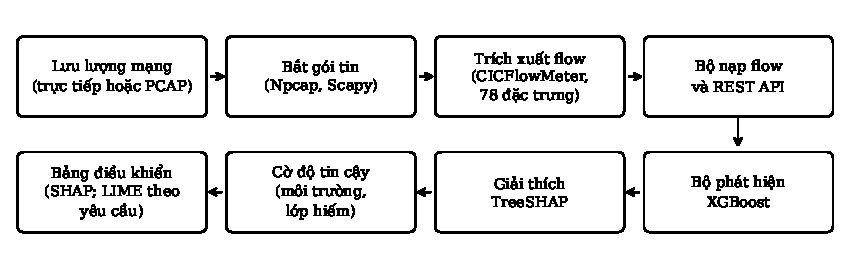
\includegraphics[width=0.92\textwidth]{figures_vi/fig2_pipeline.pdf}
\caption{Hệ thống trực tuyến. LIME chỉ chạy khi người phân tích yêu cầu.}
\label{fig:pipeline}
\end{figure*}

\subsection{Thời gian xử lý và độ trễ}
Hình~\ref{fig:latency} cho thấy thời gian xử lý của 1.025 flow và 219 cảnh báo trong một phiên thử nghiệm kết hợp nạp CSV, phát lại PCAP và bắt gói trực tiếp. Thời gian trung vị là 2,5 ms cho bước kiểm tra, 12,4 ms cho phân loại (phân vị 95 là 22,4 ms), 32,5 ms cho giá trị SHAP (40,3 ms) và 26,7 ms cho các cờ. Toàn bộ một yêu cầu mất trung vị 19,3 ms và tối đa 252,6 ms. Các tác vụ SHAP chờ trong hàng đợi trung vị 2,2 giây và tối đa 5,8 giây, vì 219 cảnh báo đến cùng lúc, phần lớn từ một lần nạp CSV.

Hệ thống làm việc ở mức flow. Một flow chỉ được phân loại sau khi bộ trích xuất đóng nó. Trong 290 flow của một phiên thực, flow trung vị kéo dài 1,35 giây, phân vị 90 là 49,0 giây và flow dài nhất là 89,9 giây. Độ trễ phát hiện vì vậy chủ yếu do thời lượng flow chứ không do xử lý, và chúng tôi gọi hệ thống là trực tuyến chứ không phải thời gian thực.

\begin{figure}[t]
\centering
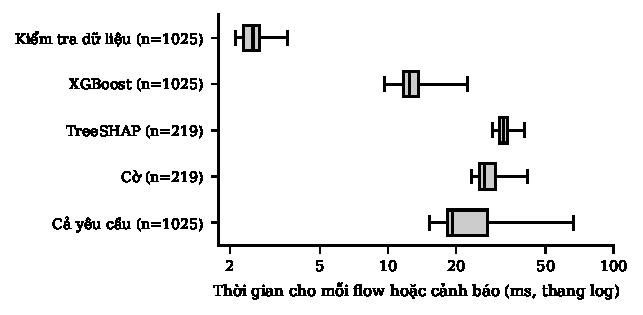
\includegraphics[width=\columnwidth]{figures_vi/fig7_latency.pdf}
\caption{Thời gian xử lý cho mỗi flow hoặc cảnh báo. Hộp thể hiện các tứ phân vị và râu thể hiện phân vị 5 và 95.}
\label{fig:latency}
\end{figure}

\subsection{Lần triển khai đầu tiên của M0 trên lưu lượng thực}
Chúng tôi chạy M0 trên 784 flow thực. M0 đưa ra cảnh báo tấn công trên 149 flow, tỷ lệ 19,01\% với khoảng Wilson 95\% từ 16,41 đến 21,90. Trong các cảnh báo này, 148 cảnh báo mang nhãn DoS-Hulk. Tỷ lệ cảnh báo khác nhau giữa bốn phiên, từ 11\% đến 59\%, và các flow trong cùng một phiên không độc lập, nên khoảng tin cậy đánh giá thấp độ bất định. Trên 21 flow duyệt web trong phòng thí nghiệm, M0 đưa ra cảnh báo trên 19 flow. Các flow này đều bình thường, nên mọi cảnh báo đều là cảnh báo sai, và điểm chuẩn 97,9\% đã không báo trước điều đó.

\subsection{Lời giải thích trên flow thực}
Giá trị TreeSHAP đạt kiểm tra cộng dồn trên cả 784 flow thực. Tổng các giá trị SHAP cộng giá trị nền khớp với đầu ra thô của mô hình với sai số tuyệt đối lớn nhất $4{,}8\times 10^{-6}$ cho M0. Đây là kiểm tra phép tính của lời giải thích. Nó không cho thấy lời giải thích giúp ích cho người phân tích.

LIME hành xử khác. Chúng tôi chạy nó trên 313 flow thật, gồm 290 flow của một phiên thực, 21 flow duyệt web và hai flow SSH. Với M0 và nền gốc, 255 flow có cỡ mẫu hiệu dụng dưới hai, nghĩa là hầu như không có mẫu nhiễu nào nằm gần flow, và chỉ hai flow qua ngưỡng chất lượng. Chúng tôi thử một cách khắc phục khả dĩ ở RQ4, khi mô hình huấn luyện lại đã có.

\textit{Trả lời RQ3.} Bộ phát hiện và lời giải thích chạy được trực tuyến, với trung vị 12,4 ms để phân loại một flow và 32,5 ms để tính giá trị SHAP, nhưng việc phát hiện bị trễ theo thời lượng flow. Lần triển khai làm lộ một lỗi của M0. M0 đưa ra cảnh báo trên 19,0\% flow thực đã xác nhận là bình thường, và LIME không cho độ khớp hợp lệ trên phần lớn chúng. RQ4 tìm nguyên nhân.

\section{RQ4: Truy nguyên lỗi về dữ liệu và kiểm chứng cách sửa}
\textit{Lý do đặt câu hỏi.} RQ3 cho thấy M0 báo động trên lưu lượng bình thường, một kết quả mà điểm chuẩn ở RQ1 không dự báo. Các cảnh báo chỉ là triệu chứng. Chúng tôi vì vậy hỏi chúng đến từ đâu, và dữ liệu huấn luyện có phải nguyên nhân không.

\subsection{SHAP chỉ về một đặc trưng}
Để thấy cái gì tạo ra các cảnh báo, chúng tôi giải thích chúng bằng SHAP, phương pháp mà RQ2 đã chọn. Chúng tôi tính giá trị TreeSHAP của đầu ra DoS-Hulk cho 148 flow thực mà M0 gán nhãn Hulk. Hình~\ref{fig:shap}a cho các giá trị trung bình. Số cờ FIN đóng góp trung bình 5,87 đơn vị log-odds, hơn gấp đôi đặc trưng kế tiếp là gói tin forward lớn nhất với 2,60. Sáu trong tám đặc trưng mạnh nhất còn lại mỗi đặc trưng đóng góp dưới 0,6 theo giá trị tuyệt đối. Hình~\ref{fig:shap}b cho cùng đại lượng của M1, mà Mục~\ref{sec:m1} bàn tới.

\begin{figure*}[t]
\centering
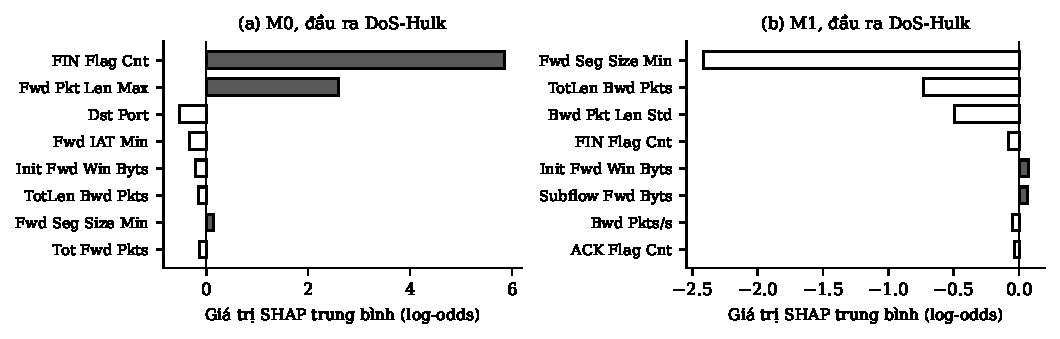
\includegraphics[width=0.92\textwidth]{figures_vi/fig4_shap.pdf}
\caption{Giá trị SHAP trung bình của đầu ra DoS-Hulk trên cùng 148 flow thực trong vùng FIN, cho (a) M0 và (b) M1. M0 gán nhãn Hulk cho cả 148 flow, còn M1 gán nhãn bình thường cho cả 148 flow.}
\label{fig:shap}
\end{figure*}

\subsection{Đường đi quyết định và vùng FIN}
\label{sec:zone}
SHAP cho một đóng góp trung bình cho từng đặc trưng nhưng không mô tả một vùng của không gian đặc trưng. Chúng tôi cần một quy tắc có thể kiểm tra trên dữ liệu khác, nên đã lần theo đường đi quyết định của một cảnh báo.

\textit{Cách xác định vùng.} Ngày 18 tháng 10 năm 2026, một cảnh báo DoS-Hulk sai từ một phiên thực có xác suất Hulk 93,3\%. Chúng tôi lần đường đi của nó qua 100 cây của lớp Hulk. Cả 100 cây đều có ít nhất một phép tách theo số cờ FIN. Trong cây có độ lợi cao nhất, cây số 38, đường đi của cảnh báo qua ba phép kiểm tra theo thứ tự. Kích thước header nhỏ nhất theo chiều đi dưới 32 byte, số cờ FIN từ một trở lên, và gói tin forward lớn nhất từ 66 byte trở lên. Chúng tôi gọi tập các flow thỏa cả ba phép kiểm tra là vùng FIN. Chúng tôi mô tả ba điều kiện trong tài liệu dự án cùng ngày và đưa vào cấu hình hệ thống ngày 20 tháng 10. Chúng đến từ một cảnh báo sai và một cây, không phải từ việc tìm kiếm trên dữ liệu.

\textit{Kiểm chứng trên dữ liệu thu sau.} Một quy tắc dựng từ một cảnh báo có thể là ngẫu nhiên, nên chúng tôi kiểm tra nó trên dữ liệu thu về sau. 784 flow thực được thu bốn ngày sau khi vùng được xác định và hai ngày sau khi nó vào cấu hình, còn tập kiểm thử nhãn đã sửa được chuẩn bị muộn hơn nữa. Không tập nào được dùng để chọn ba điều kiện. Bảng~\ref{tab:zone} cho kết quả. Trong tập flow thực, cả 148 flow trong vùng đều nhận nhãn tấn công, và 148 trong 149 cảnh báo nằm trong vùng. Điều này đúng ở cả bốn phiên. Trong tập kiểm thử bình thường có nhãn, 100.817 trong 100.849 cảnh báo nằm trong vùng, tức 99,97\%, và 100.817 trong 100.819 flow bình thường trong vùng đã bị báo. Ba điều kiện vì vậy mô tả gần hết cảnh báo sai của M0 trên cả hai tập.

\begin{table}[t]
\caption{Cảnh báo của M0 trên flow bình thường và vị trí của chúng so với vùng FIN.}
\label{tab:zone}
\centering
\footnotesize
\setlength{\tabcolsep}{4pt}
\begin{tabular}{lrrrr}
\toprule
Tập & Flow & \shortstack[r]{Trong\\vùng} & \shortstack[r]{Cảnh\\báo} & \shortstack[r]{Cảnh báo\\trong vùng} \\
\midrule
Phiên thực 1 & 34 & 19 & 20 & 19 \\
Phiên thực 2 & 32 & 19 & 19 & 19 \\
Phiên thực 3 & 242 & 27 & 27 & 27 \\
Phiên thực 4 & 476 & 83 & 83 & 83 \\
Tập thực, toàn bộ & 784 & 148 & 149 & 148 \\
\midrule
Tập kiểm thử có nhãn & 477.470 & 100.819 & 100.849 & 100.817 \\
\bottomrule
\end{tabular}
\end{table}

\subsection{Phép thử độ nhạy khi can thiệp một đặc trưng}
Giá trị SHAP lớn cho thấy mô hình nhìn vào đâu, nhưng không cho thấy nhãn phụ thuộc vào đặc trưng đó. Chúng tôi vì vậy đổi từng đặc trưng một trên 784 flow thực và đếm số flow bị đổi nhãn. Các phép thử này đo mô hình nhạy với một đặc trưng đến đâu. Chúng không mô tả những flow mà lưu lượng thật sẽ tạo ra, vì một flow đã bị sửa có thể không xuất hiện trong thực tế. Chúng không phải bằng chứng nhân quả trong lưu lượng thật. Bảng~\ref{tab:interv} cho kết quả. Đặt số cờ FIN về không đổi nhãn của cả 148 flow trong vùng, và chỉ còn bốn cảnh báo. Đặt gói tin forward lớn nhất về không cũng đổi cả 148 nhãn. Đặt header nhỏ nhất theo chiều đi lên 32 byte đổi 165 nhãn. Hai phép đối chứng, đặt cửa sổ khởi tạo theo chiều đi bằng 64.240 byte và đặt cổng đích bằng 80, chỉ đổi 1 và 5 nhãn. Ba điều kiện của vùng vì vậy mang quyết định, còn hai đặc trưng không liên quan thì không.

\begin{table}[t]
\caption{Phép thử can thiệp đặc trưng của M0 trên 784 flow thực. M0 đưa ra 149 cảnh báo trước mọi thay đổi.}
\label{tab:interv}
\centering
\footnotesize
\setlength{\tabcolsep}{3pt}
\begin{tabular}{>{\raggedright\arraybackslash}p{1.9in}>{\raggedleft\arraybackslash}p{0.6in}>{\raggedleft\arraybackslash}p{0.7in}}
\toprule
Thay đổi áp dụng cho mọi flow & Số nhãn đổi & Cảnh báo còn lại \\
\midrule
FIN Flag Cnt đặt bằng 0 & 148 & 4 \\
Fwd Pkt Len Max đặt bằng 0 & 148 & 3 \\
Fwd Seg Size Min đặt bằng 32 & 165 & 22 \\
\midrule
Init Fwd Win Byts đặt bằng 64.240 (đối chứng) & 1 & 148 \\
Dst Port đặt bằng 80 (đối chứng) & 5 & 148 \\
\bottomrule
\end{tabular}
\end{table}

\subsection{Dữ liệu huấn luyện cho thấy gì}
Nếu M0 phụ thuộc vào vùng này thì dữ liệu huấn luyện của nó phải đã dạy nó, nên chúng tôi xem dữ liệu huấn luyện chứa gì trong vùng. Hình~\ref{fig:zone} cho số flow trong vùng FIN ở hai tập huấn luyện. Trong tập huấn luyện gốc, vùng chứa 445 flow, và tất cả đều là DoS-Hulk. Với M0, vùng này là tín hiệu hoàn hảo của lớp đó. Riêng cờ FIN chưa phải toàn bộ quy tắc. Tập huấn luyện gốc có 9.815 flow bình thường với số cờ FIN khác không, nhưng không flow nào nằm trong vùng. Trong tập huấn luyện đã sửa, cùng vùng đó chứa 405.347 flow bình thường và 330 flow Hulk. Nó cũng chứa flow của các lớp tấn công khác, chẳng hạn 238.320 flow HOIC và 100.650 flow Bot, nên trong tập đó vùng không còn nhận diện riêng Hulk.

Sự khác biệt về tần suất FIN phù hợp với bức tranh này. Trong các flow huấn luyện gốc có ít nhất bốn gói mỗi chiều, chỉ 0,065\% mang cờ FIN, tức 428 trong 661.302. Trong tập huấn luyện đã sửa, 70,9\% những flow như vậy mang cờ FIN. Nghiên cứu trước báo cáo rằng bộ trích xuất gốc kết thúc một flow tại gói FIN đầu tiên trong CIC-IDS-2017 \cite{engelen2021}, và tài liệu của dữ liệu đã sửa nêu rằng cuộc tấn công Hulk trong CSE-CIC-IDS2018 cho thấy hành vi tương tự \cite{liu2022}. Kết quả của chúng tôi phù hợp với giả thuyết này, nhưng chúng tôi không kiểm tra được trên gói tin thô vì không có chúng. Chúng tôi coi bộ trích xuất là nguyên nhân có khả năng nhất chứ không phải nguyên nhân đã được chứng minh.

\begin{figure}[t]
\centering
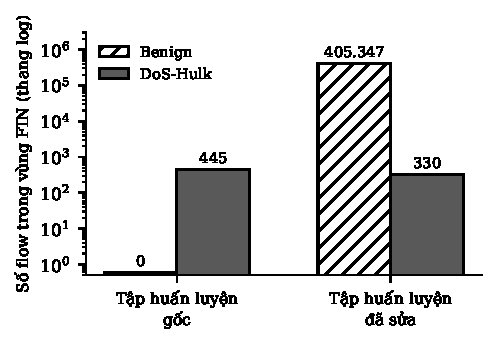
\includegraphics[width=\columnwidth]{figures_vi/fig3_zone.pdf}
\caption{Số flow Benign và DoS-Hulk trong vùng FIN ở hai tập huấn luyện. Tập đã sửa còn có flow của các lớp tấn công khác trong vùng. Tập gốc không có flow Benign nào trong vùng, và số 0 này được vẽ ở đáy của trục logarit.}
\label{fig:zone}
\end{figure}

\subsection{Huấn luyện lại trên dữ liệu đã sửa}
\label{sec:m1}
Dữ liệu huấn luyện chỉ về dữ liệu là nguyên nhân có khả năng. Để kiểm tra điều này, chúng tôi huấn luyện M1 trên dữ liệu đã sửa, có bộ trích xuất, nhãn và tập lớp khác, còn thuật toán và thiết lập giữ nguyên. Đó là phép thử của lời giải thích, nhưng nó không cho biết trong ba khác biệt này khác biệt nào quyết định. Chúng tôi đo tỷ lệ cảnh báo của cả hai mô hình trên ba tập flow bình thường, gồm phần bình thường của tập kiểm thử nhãn đã sửa với 477.470 flow, 784 flow thực và 21 flow duyệt web trong phòng thí nghiệm. Bảng~\ref{tab:alert} cho kết quả. Khoảng tin cậy là khoảng Wilson 95\%, và cận trên cho trường hợp không có cảnh báo là cận Clopper-Pearson. M0 đưa ra cảnh báo trên 21,12\% flow trong tập kiểm thử bình thường có nhãn, so với 0,23\% trên tập kiểm thử của chính nó. M1 đưa ra 7 cảnh báo trên tập kiểm thử bình thường có nhãn và không cảnh báo nào trên các flow thực và flow duyệt web.

\begin{table*}[t]
\caption{Tỷ lệ cảnh báo trên flow bình thường, kèm khoảng tin cậy 95\%. M0 huấn luyện trên dữ liệu gốc và M1 trên dữ liệu đã sửa.}
\label{tab:alert}
\centering
\small
\begin{tabular}{lrcc}
\toprule
Tập flow bình thường & Flow & Cảnh báo của M0 (tỷ lệ, khoảng) & Cảnh báo của M1 (tỷ lệ, khoảng) \\
\midrule
Tập kiểm thử có nhãn, nhãn đã sửa & 477.470 & 100.849 (21,12\%, 21,01 đến 21,24) & 7 (0,0015\%, 0,0007 đến 0,0030) \\
Lưu lượng thực, đã xác nhận bình thường & 784 & 149 (19,01\%, 16,41 đến 21,90) & 0 (0,00\%, cận trên 0,47) \\
Duyệt web trong phòng thí nghiệm & 21 & 19 (90,48\%, 71,09 đến 97,35) & 0 (0,00\%, cận trên 16,11) \\
\bottomrule
\end{tabular}
\end{table*}

Cả 148 flow thực trong vùng FIN đều nhận nhãn bình thường từ M1. Hình~\ref{fig:shap}b cho thấy vì sao. Với đầu ra Hulk của M1, số cờ FIN chỉ đóng góp trung bình $-0{,}08$, và đặc trưng mạnh nhất là kích thước header nhỏ nhất theo chiều đi, với $-2{,}42$, đẩy quyết định ra xa Hulk. M1 dùng một đặc trưng khác thay cho FIN, và đặc trưng đó cũng phụ thuộc vào hệ điều hành.

\textit{Điểm chuẩn của M1.} M1 đạt độ chính xác 99,996\% và macro F1 99,30\% trên tập kiểm thử chia ngẫu nhiên của nó. Con số này cao hơn mọi điểm của M0, và điểm cao như vậy cần được kiểm tra, vì nó có thể đến từ các dòng trùng hoặc từ một cách chia dễ. Chúng tôi kiểm tra điểm này bằng phép chia theo khối thời gian, đếm dòng trùng và các mốc so sánh đơn giản. Với phép chia theo khối thời gian, chúng tôi cắt mỗi lớp thành năm khối thời gian liên tục, huấn luyện trên bốn khối với khoảng đệm 1\% ở hai đầu khối kiểm thử, và kiểm thử trên khối thứ năm (Hình~\ref{fig:blocked}). Macro F1 dao động từ 98,1\% đến 99,99\% qua các khối, và tỷ lệ cảnh báo trên flow bình thường từ 0,0015\% đến 0,0034\%. Trong phép chia ngẫu nhiên, 115.467 trong 682.100 dòng kiểm thử, tức 16,9\%, cũng xuất hiện trong tập huấn luyện, và loại chúng đi vẫn để độ chính xác ở 99,996\%. Trên dữ liệu này, một bộ phân loại luôn trả lời bình thường đạt độ chính xác 70,0\%, một cây quyết định độ sâu ba đạt 96,4\%, và một mô hình huấn luyện trên 0,1\% dữ liệu huấn luyện đạt độ chính xác 99,76\% và macro F1 96,63\%. Bộ chuẩn này dễ. Điểm của nó không dự báo hiệu năng ngoài thực tế.

\begin{figure}[t]
\centering
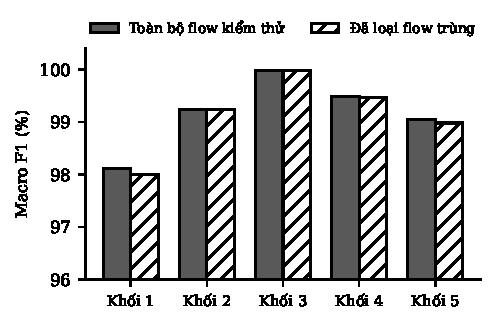
\includegraphics[width=\columnwidth]{figures_vi/fig5_blocked.pdf}
\caption{Đánh giá theo khối thời gian của M1 trên dữ liệu đã sửa.}
\label{fig:blocked}
\end{figure}

\textit{Hai flow SSH.} Hai flow brute force SSH, mỗi file một flow, quá ít để ước lượng tỷ lệ phát hiện. M1 gán nhãn SSH-Bruteforce cho cả hai, với độ tin cậy 0,82 và 0,78, còn M0 gán nhãn DoS-Hulk cho cả hai, tức một nhãn tấn công sai lớp. Chúng tôi chỉ báo cáo chúng như một kiểm tra rằng M1 không gán nhãn bình thường cho mọi thứ. Cả hai đến từ một máy tấn công và một máy nạn nhân trong một phòng thí nghiệm, và mỗi flow là một kết nối dài.

\subsection{LIME một lần nữa, với mô hình huấn luyện lại}
RQ3 để lại một câu hỏi mở. LIME thất bại trên phần lớn flow thật với M0 và nền gốc. Khi đã có M1, chúng tôi hỏi liệu thất bại có đến từ nền hay không. Chúng tôi kỳ vọng nền lấy từ dữ liệu đã sửa sẽ giúp ích, nên chạy LIME với M1 và nền gồm 2.000 flow huấn luyện đã sửa trên cùng 313 flow thật. Cả 313 flow có cỡ mẫu hiệu dụng dưới hai, và không flow nào qua ngưỡng chất lượng (Hình~\ref{fig:lime}). Tỷ lệ qua ngưỡng trên nhóm kiểm thử 1.339 flow, 86,0\%, và trên 100 flow bình thường của nhóm đó, 23,0\%, được vẽ để so sánh. Trong thiết lập này LIME không cho độ khớp cục bộ hợp lệ trên flow thật, với cả hai mô hình. Chúng tôi không thử các độ rộng kernel hoặc cỡ mẫu khác, nên kết quả không áp dụng cho LIME nói chung. Giá trị TreeSHAP cũng đạt kiểm tra cộng dồn trên cả 784 flow với M1, với sai số lớn nhất $3{,}8\times 10^{-6}$.

\begin{figure*}[t]
\centering
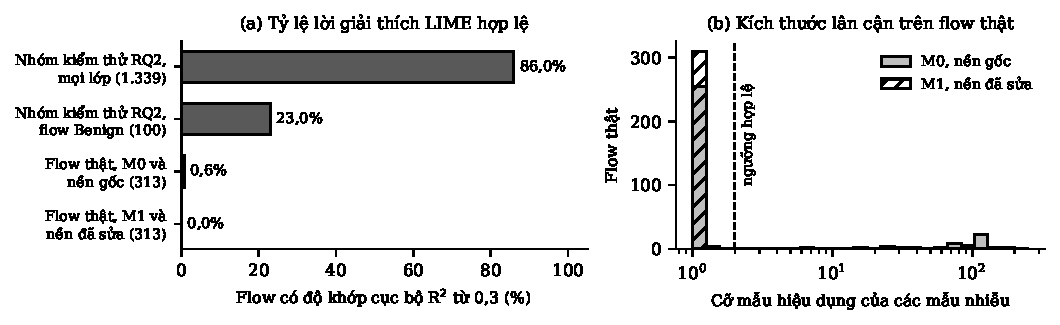
\includegraphics[width=0.92\textwidth]{figures_vi/fig6_lime.pdf}
\caption{Độ hợp lệ của lời giải thích LIME. (a) Tỷ lệ lời giải thích có độ khớp cục bộ $R^2\ge 0{,}3$. (b) Cỡ mẫu hiệu dụng của các mẫu nhiễu trên 313 flow thật. Giá trị dưới hai làm độ khớp không hợp lệ.}
\label{fig:lime}
\end{figure*}

\textit{Trả lời RQ4.} Có, ở vế thứ nhất. SHAP, vết đường đi quyết định và các phép thử can thiệp đặc trưng đã gắn lỗi với một vùng ba điều kiện quanh số cờ FIN, và vùng đó chỉ chứa flow Hulk trong dữ liệu huấn luyện gốc. Huấn luyện lại trên dữ liệu đã sửa loại bỏ lỗi trên các flow bình thường của chúng tôi, nhưng bộ chuẩn đã sửa dễ, và nguyên nhân của lối tắt vẫn là một giả thuyết.

\section{Thảo luận và hạn chế}
Chúng tôi tách các kết luận thành ba mức.

\textit{Điều dữ liệu cho thấy.} M0 dùng một vùng của không gian đặc trưng mà trong dữ liệu huấn luyện chỉ chứa flow DoS-Hulk, và vùng này chứa gần hết cảnh báo sai của nó trên các flow thực và trên các flow bình thường có nhãn. Biểu đồ SHAP của các cảnh báo sai chỉ về số cờ FIN, và vết đường đi quyết định biến điều đó thành ba điều kiện. Mô hình huấn luyện lại M1 không đưa ra cảnh báo nào trên 784 flow thực và 21 flow duyệt web.

\textit{Điều dữ liệu hỗ trợ nhưng chưa chứng minh.} Lối tắt nhiều khả năng đến từ một bộ trích xuất kết thúc flow tại gói FIN đầu tiên. Bằng chứng của chúng tôi là nội dung của vùng trong dữ liệu huấn luyện, khác biệt về tần suất FIN và các báo cáo trước về bộ trích xuất. Chúng tôi không kiểm tra bộ trích xuất trên gói tin thô. Các phép thử can thiệp đặc trưng cho thấy mô hình nhạy với một đặc trưng đến đâu, và không cho thấy lưu lượng thật trông ra sao.

\textit{Điều còn bỏ ngỏ.} Chưa biết M1 có phát hiện được tấn công trong một mạng thật hay không, vì bằng chứng tấn công của chúng tôi là hai flow SSH. M1 thay mẫu FIN bằng một mẫu kích thước header cũng phụ thuộc vào hệ điều hành, và bộ chuẩn của nó chứa các flow gần trùng nhau. Chúng tôi không báo cáo M1 trên miền gốc. Kết quả LIME của chúng tôi có đúng trong các thiết lập khác hay không cũng chưa rõ.

Dữ liệu còn bị giới hạn theo những cách khác. Tập thực đến từ một máy tính trong bốn phiên, nhãn bình thường của nó dựa vào lời xác nhận của chúng tôi mà không có nhật ký hoạt động, và các flow trong một phiên có tương quan với nhau. Chúng tôi loại các bản bắt gói khác trong phòng thí nghiệm vì không kiểm chứng được nhãn. Chúng tôi chỉ thử XGBoost và một bộ dữ liệu đã sửa. Các cờ độ tin cậy của hệ thống chưa được kiểm chứng, và chúng tôi không thực hiện nghiên cứu nào với người phân tích.

Từ trường hợp này có một quy tắc thực hành. Trước khi triển khai, hãy chạy bộ phân loại trên một tập nhỏ lưu lượng bình thường của mạng đích và xem lời giải thích của từng cảnh báo sai.

\section{Kết luận}
Chúng tôi xây dựng một bộ phát hiện xâm nhập trực tuyến qua bốn bước. Ở RQ1, một bộ phân loại XGBoost đạt độ chính xác 97,9\% trên CSE-CIC-IDS2018. Ở RQ2, SHAP trung thực và ổn định hơn LIME. Ở RQ3, bộ phân loại được triển khai đã đưa ra cảnh báo trên 19,0\% trong 784 flow thực mà chúng tôi xác nhận là bình thường. Ở RQ4, giá trị SHAP, vết đường đi quyết định và các phép thử can thiệp đặc trưng đã xác định một vùng ba điều kiện quanh số cờ FIN. Vùng đó chứa 148 trong 149 cảnh báo và 99,97\% cảnh báo sai trên một tập bình thường lớn có nhãn, và trong dữ liệu huấn luyện gốc nó chỉ chứa flow DoS-Hulk. Dữ liệu phù hợp với một bộ trích xuất kết thúc flow tại gói FIN đầu tiên, điều chúng tôi không kiểm chứng được trên gói tin thô. Bộ phân loại huấn luyện trên dữ liệu đã sửa không đưa ra cảnh báo nào trên các flow thực, nhưng bộ chuẩn của nó dễ và điểm của nó không nên đọc như hiệu năng ngoài thực tế. Trong cấu hình đã thử, LIME không cho độ khớp hợp lệ trên flow thật, còn TreeSHAP đạt kiểm tra cộng dồn trên tất cả. Công việc tiếp theo cần thu lưu lượng tấn công có nhãn trong một mạng thật, kiểm tra bộ trích xuất trên gói tin thô, và kiểm tra xem các cờ độ tin cậy có dự báo được những lời giải thích làm người phân tích hiểu sai hay không.

\appendices
\section{Danh mục dữ liệu và tệp}
Bảng~\ref{tab:inventory} liệt kê dữ liệu, phần mềm và hạt giống ngẫu nhiên của các thí nghiệm. Chúng tôi không ghi lại mã phiên bản của bộ dữ liệu đã sửa, nên bảng chỉ cho ngày chúng tôi lấy về.

\begin{table}[h]
\caption{Dữ liệu, phần mềm và hạt giống ngẫu nhiên.}
\label{tab:inventory}
\centering
\footnotesize
\setlength{\tabcolsep}{3pt}
\begin{tabular}{>{\raggedright\arraybackslash}p{1.0in}>{\raggedright\arraybackslash}p{2.25in}}
\toprule
Mục & Giá trị \\
\midrule
Dữ liệu gốc & Các file CSV đã xử lý của CSE-CIC-IDS2018 từ kho AWS công khai. 15.589.784 flow đã làm sạch nằm trong mười file Parquet theo ngày \\
Dữ liệu đã sửa & Bộ dữ liệu dựng lại của Liu và cộng sự, mười file CSV theo ngày, lấy về ngày 22 tháng 10 năm 2026 \\
Bộ trích xuất flow & CICFlowMeter bản Python 0.5.0 với phiên bản vòng đời của dự án rq3-cfm-0.5.0-lifecycle-v3, Scapy 2.8.0, Npcap 1.89 \\
Phần mềm & Python 3.14.7, XGBoost 3.4.1, SHAP 0.52.0, LIME 0.2.0.1, scikit-learn 1.9.1, pandas 3.0.6 \\
Hạt giống ngẫu nhiên & Chia dữ liệu và XGBoost dùng hạt giống 42. Ba lần chia lại dùng các hạt giống 1, 2 và 3. LIME dùng nền 2.000 flow lấy với hạt giống 42 và một hạt giống suy ra riêng cho từng flow \\
\bottomrule
\end{tabular}
\end{table}

\balance
\bibliographystyle{IEEEtran}
\bibliography{refs}

\end{document}
